%!LW recipe=LuaLaTeX (latexmk)

\documentclass[final]{beamer}

% ====================
% Packages
% ====================
\usepackage[size=custom,width=120,height=90,scale=1.0]{beamerposter}
% \usepackage[T1]{fontenc}
\usepackage{lmodern}
\usepackage{lipsum}
\usepackage{raleway}   % Load raleway font
\usetheme{gemini}
\usecolortheme{gemini}
%\usepackage{graphicx}
% \usepackage{booktabs}
%\usepackage[utf8]{inputenc}
\usepackage{qrcode} % If you want to include a QR code to your paper
\usepackage{mathtools}
\usepackage{amsmath,amssymb,amsfonts,amsthm}
\usepackage{tikz}
\usetikzlibrary{overlay-beamer-styles}
\usepackage{pgfplots} 
\usetikzlibrary{shapes}
\pgfplotsset{compat=newest} 
\pgfplotsset{plot coordinates/math parser=false} 
\usepackage{subcaption}
\usepackage{multirow}
\usepackage[backend=biber,style=numeric,sorting=none, maxnames=99]{biblatex}
\usepackage{colortbl}
\usepackage{arydshln}
\addbibresource{bibliography.bib} % Replace with your .bib file
% \usepackage{tikz-imagelabels}
% \usepackage{pgfgantt}
% \usepackage{pdflscape}
% \newlength\fwidth
% \newlength\fheight
\definecolor{ucsdblue}{RGB}{1, 49, 82}

%%% Kronecker product power notation
\newcommand*\circled[1]{\tikz[baseline=(char.base)]{\node(char)[shape=rounded rectangle,draw,inner sep=0.6pt,minimum height=1.5ex]{#1};}} % 
\newcommand\kronF[2]{{#1}^{\circled{\small{\ensuremath{#2}}}}} % Kronecker
\renewcommand\Vec[1][]{\text{vec}\ensuremath{\if$#1$ \else \left[#1\right]\fi}}

\newcommand{\bzero}{\ensuremath{\mathbf{0}}} % Bold zero often needed

% %%%% \tilde letters
\newcommand{\tA}{\ensuremath{\tilde{A}}}
\newcommand{\tB}{\ensuremath{\tilde{B}}}
\newcommand{\tC}{\ensuremath{\tilde{C}}}
\newcommand{\tD}{\ensuremath{\tilde{D}}}
\newcommand{\tE}{\ensuremath{\tilde{E}}}
\newcommand{\tF}{\ensuremath{\tilde{F}}}
\newcommand{\tG}{\ensuremath{\tilde{G}}}
\newcommand{\tH}{\ensuremath{\tilde{H}}}
\newcommand{\tI}{\ensuremath{\tilde{I}}}
\newcommand{\tJ}{\ensuremath{\tilde{J}}}
\newcommand{\tK}{\ensuremath{\tilde{K}}}
\newcommand{\tL}{\ensuremath{\tilde{L}}}
\newcommand{\tM}{\ensuremath{\tilde{M}}}
\newcommand{\tN}{\ensuremath{\tilde{N}}}
\newcommand{\tO}{\ensuremath{\tilde{O}}}
\newcommand{\tP}{\ensuremath{\tilde{P}}}
\newcommand{\tQ}{\ensuremath{\tilde{Q}}}
\newcommand{\tR}{\ensuremath{\tilde{R}}}
\newcommand{\tS}{\ensuremath{\tilde{S}}}
\newcommand{\tT}{\ensuremath{\tilde{T}}}
\newcommand{\tU}{\ensuremath{\tilde{U}}}
\newcommand{\tV}{\ensuremath{\tilde{V}}}
\newcommand{\tW}{\ensuremath{\tilde{W}}}
\newcommand{\tX}{\ensuremath{\tilde{X}}}
\newcommand{\tY}{\ensuremath{\tilde{Y}}}
\newcommand{\tZ}{\ensuremath{\tilde{Z}}}
\newcommand{\tSigma}{\ensuremath{\tilde{\Sigma}}}
%
\newcommand{\ta}{\ensuremath{\tilde{a}}}
\newcommand{\tb}{\ensuremath{\tilde{b}}}
\newcommand{\tc}{\ensuremath{\tilde{c}}}
\newcommand{\td}{\ensuremath{\tilde{d}}}
\newcommand{\te}{\ensuremath{\tilde{e}}}
\newcommand{\tf}{\ensuremath{\tilde{f}}}
\newcommand{\tg}{\ensuremath{\tilde{g}}}
\newcommand{\tth}{\ensuremath{\tilde{h}}}
\newcommand{\ti}{\ensuremath{\tilde{i}}}
\newcommand{\tj}{\ensuremath{\tilde{j}}}
\newcommand{\tk}{\ensuremath{\tilde{k}}}
\newcommand{\tl}{\ensuremath{\tilde{l}}}
\newcommand{\tm}{\ensuremath{\tilde{m}}}
\newcommand{\tn}{\ensuremath{\tilde{n}}}
\newcommand{\tto}{\ensuremath{\tilde{o}}}
\newcommand{\tp}{\ensuremath{\tilde{p}}}
\newcommand{\tq}{\ensuremath{\tilde{q}}}
\newcommand{\tr}{\ensuremath{\tilde{r}}}
\newcommand{\tss}{\ensuremath{\tilde{s}}}
\newcommand{\ttt}{\ensuremath{\tilde{t}}}
\newcommand{\tu}{\ensuremath{\tilde{u}}}
\newcommand{\tv}{\ensuremath{\tilde{v}}}
\newcommand{\tw}{\ensuremath{\tilde{w}}}
\newcommand{\tx}{\ensuremath{\tilde{x}}}
\newcommand{\ty}{\ensuremath{\tilde{y}}}
\newcommand{\tz}{\ensuremath{\tilde{z}}}

%%% bold letters
\newcommand{\bA}{\ensuremath{\mathbf{A}}}
\newcommand{\bB}{\ensuremath{\mathbf{B}}}
\newcommand{\bC}{\ensuremath{\mathbf{C}}}
\newcommand{\bD}{\ensuremath{\mathbf{D}}}
\newcommand{\bE}{\ensuremath{\mathbf{E}}}
\newcommand{\bF}{\ensuremath{\mathbf{F}}}
\newcommand{\bG}{\ensuremath{\mathbf{G}}}
\newcommand{\bH}{\ensuremath{\mathbf{H}}}
\newcommand{\bI}{\ensuremath{\mathbf{I}}}
\newcommand{\bJ}{\ensuremath{\mathbf{J}}}
\newcommand{\bK}{\ensuremath{\mathbf{K}}}
\newcommand{\bL}{\ensuremath{\mathbf{L}}}
\newcommand{\bM}{\ensuremath{\mathbf{M}}}
\newcommand{\bN}{\ensuremath{\mathbf{N}}}
\newcommand{\bO}{\ensuremath{\mathbf{O}}}
\newcommand{\bP}{\ensuremath{\mathbf{P}}}
\newcommand{\bQ}{\ensuremath{\mathbf{Q}}}
\newcommand{\bR}{\ensuremath{\mathbf{R}}}
\newcommand{\bS}{\ensuremath{\mathbf{S}}}
\newcommand{\bT}{\ensuremath{\mathbf{T}}}
\newcommand{\bU}{\ensuremath{\mathbf{U}}}
\newcommand{\bV}{\ensuremath{\mathbf{V}}}
\newcommand{\bW}{\ensuremath{\mathbf{W}}}
\newcommand{\bX}{\ensuremath{\mathbf{X}}}
\newcommand{\bY}{\ensuremath{\mathbf{Y}}}
\newcommand{\bZ}{\ensuremath{\mathbf{Z}}}

\newcommand{\ba}{\ensuremath{\mathbf{a}}}
\newcommand{\bb}{\ensuremath{\mathbf{b}}}
\newcommand{\bc}{\ensuremath{\mathbf{c}}}
\newcommand{\bd}{\ensuremath{\mathbf{d}}}
\newcommand{\be}{\ensuremath{\mathbf{e}}}
\renewcommand{\bf}{\ensuremath{\mathbf{f}}}
\newcommand{\bg}{\ensuremath{\mathbf{g}}}
\newcommand{\bh}{\ensuremath{\mathbf{h}}}
\newcommand{\bi}{\ensuremath{\mathbf{i}}}
\newcommand{\bj}{\ensuremath{\mathbf{j}}}
\newcommand{\bk}{\ensuremath{\mathbf{k}}}
\newcommand{\bl}{\ensuremath{\mathbf{l}}}
\newcommand{\bm}{\ensuremath{\mathbf{m}}}
\newcommand{\bn}{\ensuremath{\mathbf{n}}}
\newcommand{\bo}{\ensuremath{\mathbf{o}}}
\newcommand{\bp}{\ensuremath{\mathbf{p}}}
\newcommand{\bq}{\ensuremath{\mathbf{q}}}
\newcommand{\br}{\ensuremath{\mathbf{r}}}
\newcommand{\bt}{\ensuremath{\mathbf{t}}}
\newcommand{\bu}{\ensuremath{\mathbf{u}}}
\newcommand{\bv}{\ensuremath{\mathbf{v}}}
\newcommand{\bw}{\ensuremath{\mathbf{w}}}
\newcommand{\bx}{\ensuremath{\mathbf{x}}}
\newcommand{\by}{\ensuremath{\mathbf{y}}}
\newcommand{\bz}{\ensuremath{\mathbf{z}}}

%%%% bold greek letters (requires amsmath}
\newcommand{\balpha}{\ensuremath{\mbox{\boldmath $\alpha$}}}
\newcommand{\bbeta}{\ensuremath{\mbox{\boldmath $\beta$}}}
\newcommand{\bgamma}{\mbox{\boldmath $\gamma$}}
\newcommand{\blambda}{\mbox{\boldmath $\lambda$}}
\newcommand{\bLambda}{\mbox{\boldmath $\Lambda$}}
\newcommand{\bepsilon}{\mbox{\boldmath $\epsilon$}}
\newcommand{\bGamma}{\boldsymbol{\Gamma}}
\newcommand{\bOmega}{\boldsymbol{\Omega}}
\newcommand{\bpsi}{\mbox{\boldmath $\psi$}}
\newcommand{\bPsi}{\mbox{\boldmath $\Psi$}}
\newcommand{\bphi}{\mbox{\boldmath $\phi$}}
\newcommand{\bPhi}{\mbox{\boldmath $\Phi$}}
\newcommand{\bet}{\mbox{\boldmath $\eta$}}
\newcommand{\bpi}{\mbox{\boldmath $\pi$}}
\newcommand{\bxi}{\mbox{\boldmath $\xi$}}
\newcommand{\bPi}{\mbox{\boldmath $\Pi$}}
\newcommand{\btheta}{\mbox{\boldmath $\theta$}}
\newcommand{\bsigma}{\ensuremath{\boldsymbol{\sigma}}}
\newcommand{\bSigma}{\ensuremath{\boldsymbol{\Sigma}}}

%%%% caligraphic letters
\newcommand{\cA}{\ensuremath{\mathcal{A}}}
\newcommand{\cB}{\ensuremath{\mathcal{B}}}
\newcommand{\cC}{\ensuremath{\mathcal{C}}}
\newcommand{\cD}{\ensuremath{\mathcal{D}}}
\newcommand{\cE}{\ensuremath{\mathcal{E}}}
\newcommand{\cF}{\ensuremath{\mathcal{F}}}
\newcommand{\cG}{\ensuremath{\mathcal{G}}}
\newcommand{\cH}{\ensuremath{\mathcal{H}}}
\newcommand{\cI}{\ensuremath{\mathcal{I}}}
\newcommand{\cJ}{\ensuremath{\mathcal{J}}}
\newcommand{\cK}{\ensuremath{\mathcal{K}}}
\newcommand{\cL}{\ensuremath{\mathcal{L}}}
\newcommand{\cM}{\ensuremath{\mathcal{M}}}
\newcommand{\cN}{\ensuremath{\mathcal{N}}}
\newcommand{\cO}{\ensuremath{\mathcal{O}}}
\newcommand{\cP}{\ensuremath{\mathcal{P}}}
\newcommand{\cQ}{\ensuremath{\mathcal{Q}}}
\newcommand{\cR}{\ensuremath{\mathcal{R}}}
\newcommand{\cS}{\ensuremath{\mathcal{S}}}
\newcommand{\cT}{\ensuremath{\mathcal{T}}}
\newcommand{\cU}{\ensuremath{\mathcal{U}}}
\newcommand{\cV}{\ensuremath{\mathcal{V}}}
\newcommand{\cW}{\ensuremath{\mathcal{W}}}
\newcommand{\cX}{\ensuremath{\mathcal{X}}}
\newcommand{\cY}{\ensuremath{\mathcal{Y}}}
\newcommand{\cZ}{\ensuremath{\mathcal{Z}}}

\newcommand{\ca}{\ensuremath{\mathcal{a}}}
\newcommand{\cb}{\ensuremath{\mathcal{b}}}
\newcommand{\cd}{\ensuremath{\mathcal{d}}}
\newcommand{\ce}{\ensuremath{\mathcal{e}}}
\newcommand{\cf}{\ensuremath{\mathcal{f}}}
\newcommand{\cg}{\ensuremath{\mathcal{g}}}
\newcommand{\ch}{\ensuremath{\mathcal{h}}}
\newcommand{\ci}{\ensuremath{\mathcal{i}}}
\newcommand{\cj}{\ensuremath{\mathcal{j}}}
\newcommand{\cm}{\ensuremath{\mathcal{m}}}
\newcommand{\cn}{\ensuremath{\mathcal{n}}}
\newcommand{\co}{\ensuremath{\mathcal{o}}}
\newcommand{\cp}{\ensuremath{\mathcal{p}}}
\newcommand{\cq}{\ensuremath{\mathcal{q}}}
\newcommand{\cs}{\ensuremath{\mathcal{s}}}
\newcommand{\ct}{\ensuremath{\mathcal{t}}}
\newcommand{\cu}{\ensuremath{\mathcal{u}}}
\newcommand{\cv}{\ensuremath{\mathcal{v}}}
\newcommand{\cw}{\ensuremath{\mathcal{w}}}
\newcommand{\cx}{\ensuremath{\mathcal{x}}}
\newcommand{\cy}{\ensuremath{\mathcal{y}}}
\newcommand{\cz}{\ensuremath{\mathcal{z}}}

%%% More macros
\newcommand{\ra}{\text{a}}
\newcommand{\rb}{\text{b}}
\newcommand{\rc}{\text{c}}
\newcommand{\rd}{\text{d}}

% ====================
% Lengths
% ====================

% If you have N columns, choose \sepwidth and \colwidth such that
% (N+1)*\sepwidth + N*\colwidth = \paperwidth
\newlength{\sepwidth}
\newlength{\colwidth}
\setlength{\sepwidth}{0.025\paperwidth}
\setlength{\colwidth}{0.3\paperwidth}

\newcommand{\separatorcolumn}{\begin{column}{\sepwidth}\end{column}}

% ====================
% Title
% ====================

\title{Discovering Quadratic Representations of PDEs:
Algorithms and Software}

\author[1]{Albani Olivieri \inst{1}
\and Gleb Pogudin \inst{2}
\and Boris Kramer \inst{1}}

\institute[shortinst]{\inst{1} Department of 
Mechanical and Aerospace Engineering, University of California San Diego
\inst{2} LIX, CNRS, \'Ecole Polytechnique, Institute Polytechnique de Paris}

% ====================
% Body
% ====================

\begin{document}

\Large


\addtobeamertemplate{headline}{}
{ % if these don't appear on your local latex compiler, try the commented out ones at the end of the file
  \begin{tikzpicture}[remember picture,overlay]
    \node [shift={(11 cm,-8cm)}] at (current page.north west) {
\includegraphics[height=4.5cm]{figures/UCSDLogo_JSOE_White.png}};
    \node [shift={(-7cm,-5.7cm)}] at (current page.north east) {
\includegraphics[height=10cm]{figures/UCSD_logo.png}};
  \end{tikzpicture}

}
\begin{frame}[t]
  \begin{columns}[t]
    \separatorcolumn

    \begin{column}{0.96\colwidth}
      % \begin{block}{What Is A Thought Provoking Question?}
      %   \begin{center}
      %     % We can put pictures in without a figure environment if we don't need a caption
      %     % \includegraphics[width=.5\linewidth]{example-grid-100x100pt}
      %   \end{center}
      %   \vspace{-2cm}
      % \end{block}
    
      \begin{block}{Background and Motivation}
      \vspace{-0.2cm}
        \begin{itemize}
          \item Nonpolynomial and nonquadratic PDEs describe complex dynamical processes in science and engineering. 
          \item Lifting PDE systems to quadratic form before applying MOR techniques can yield better results, see \cite{GU2011, LIFTING2019, LIFT&LEARN}. 
          
          
          \begin{center}
              
                  \begin{tikzpicture}
                    % Define nodes
                    \node (A) at (0,0) [align=center] {Nonquadratic PDE\\$\textbf{u}{_t} = \textbf{f}(\textbf{u},\mathcal{D}_{\textbf{u}})$};
                    \node (B) at (13,0) [align=center]{\textbf{Quadratic} \textbf{PDE}\\$\hat{\textbf{u}}{_t} = \hat{\textbf{f}}(\textbf{u}, \mathcal{D}_{\textbf{u}})$\\$\textbf{w}{_t} = \hat{\textbf{q}}(\textbf{u}, \mathcal{D}_{\textbf{u}})$};
                    \node (C) at (25,0) [align=center] {Reduced\\model};
                    
                    % Draw arrows with text under them
                    \draw[->, >=stealth, line width=5pt] (A) -- (B) node[midway, below, align=center] {\normalsize lifting};
                    \draw[->, line width=5pt] (B) -- (C) node[midway, below, align=center] {$\substack{\text{MOR}\\ \text{technique}}$};
                \end{tikzpicture}
          \end{center}

          \item No algorithmic tool exists to do this lifting directly for PDEs. 
        \end{itemize}
      \end{block}
      \vspace{-0.7cm}
      \begin{alertblock}{Research Problem}
        % We ask ourselves the following questions:
        \begin{center}
        Design an algorithm that finds quadratic liftings/transformations for PDEs.
        \end{center}
      \end{alertblock}
        \vspace{-0.7cm}
      \begin{block}{Example: Quadratization for a PDE}
      \vspace{-0.2cm}

          \begin{enumerate}
              \item Consider a nonquadratic PDE for $u(t,x)$:
              \begin{equation}
              \label{eq:pde-ex-1}
                  u_t = u_xu^2.
              \end{equation}
              \item We introduce a new variable with its partial derivative in $x$:
              \begin{equation*}
                  y = u^2 \hspace{1.5cm} \Rightarrow \hspace{1.5cm} y_x = 2u_xu.
              \end{equation*}
              \item We re-write the original PDE and add a differential equation corresponding to the new variable:
              \begin{align*}
                  & u_t = u_xy \\
                  & y_t = y_xy.
              \end{align*}
          \end{enumerate}
          The set $\{u^2\}$ is called a monomial quadratization for Eq.~\eqref{eq:pde-ex-1}.
        
      \end{block}
      \vspace{-0.7cm}
      \begin{alertblock}{Research Problem}
    % We ask ourselves the following questions:
    \begin{center} 
    
    Can we find monomial quadratizations quickly and ensure optimality, i.e., that we add the least number of variables?
    \end{center}
  \end{alertblock}      

      \begin{block}{Algorithm \textit{QuPDE} (Quadratization for Partial Differential Equations)}
      \textcolor{ucsdblue}{\textbf{A)} \underline{\textbf{Which lifting variables should the algorithm suggest?}}}
          
        \vspace{0.8cm}
        
        Monomial decomposition: How many ways can we divide a set of elements of size $n$ into two subsets? 
      
      \begin{figure}
        \centering
        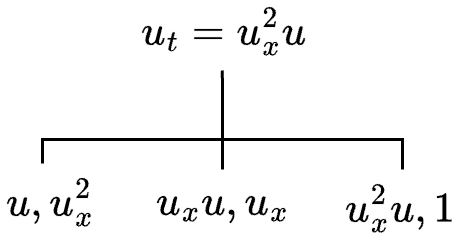
\includegraphics[width=0.45\linewidth]{figures/decomp_examples.png}
        \label{fig:decomp}
      \end{figure}
    The new variable candidates would be $\{u_x^2, u_xu, u_x^2u\}$.

    \end{block}

  
    \end{column}

    \separatorcolumn

    \begin{column}{1.01\colwidth}

         \textcolor{ucsdblue}{\textbf{B)} \underline{\textbf{How can we automate the search for the best quadratization?}}}

    \begin{enumerate}
        \item \textbf{Branch-and-Bound (B\&B)} 
        
        For each node (set) that is not a quadratization, we add as children all the subproblems that come from the transformed PDE of the parent node. If we consider the example PDE:
        \vspace{0.5cm}
        \begin{equation}
            \Large u_t = u_x^3 + u^3,
        \end{equation}
        
        \vspace{0.7cm}
        
        its search tree for finding a quadratization is:
        \begin{figure}
        \centering
        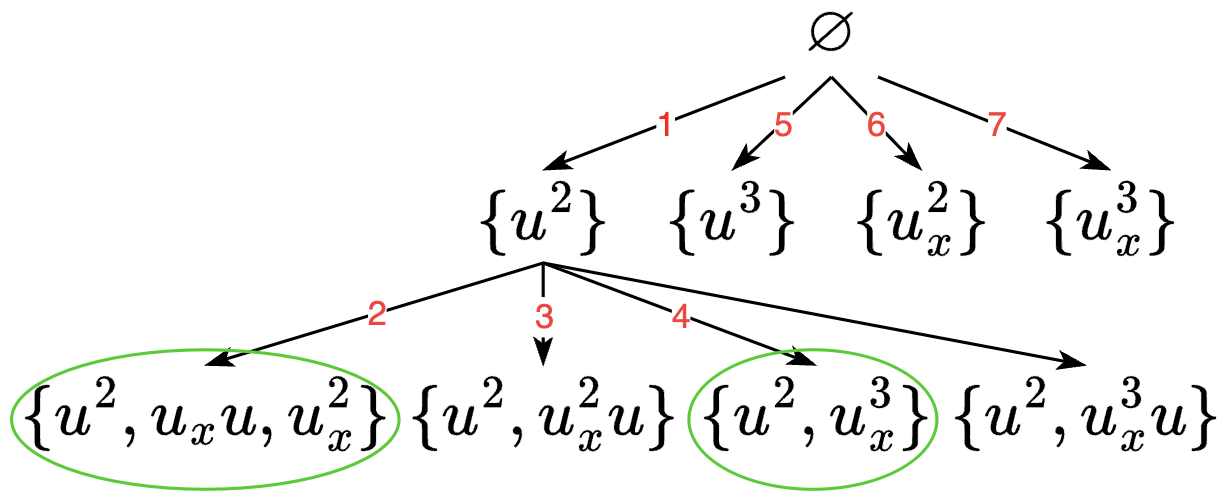
\includegraphics[width=0.85\linewidth]{figures/b&bfull_path.png}
        \label{fig:b&b}
      \end{figure}
      \item \textbf{Incremental Nearest Neighbor (INN)} 
      
      In each iteration, we check whether the best set stored so far is a quadratization. If not, we store all its subproblems. For the PDE:
      \vspace{0.5cm}
      \begin{equation}
          u_t = u_x^4
      \end{equation}
      
      \vspace{0.7cm}
      
      this algorithm would do the following:
      \begin{figure}
        \centering
        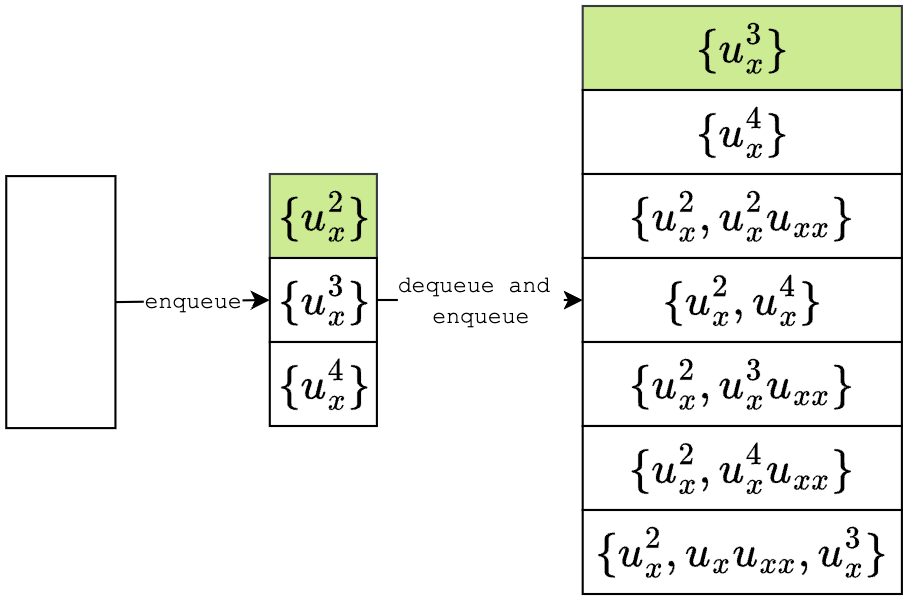
\includegraphics[width=0.85\linewidth]{figures/full_nearest_neighbor.png}
        \label{fig:nn}
      \end{figure}
        
    \end{enumerate}
        \textcolor{ucsdblue}{\textbf{C)} \underline{\textbf{How can we check if a set is a quadratization?}}}
        
        Consider the sets: 
        \vspace{-0.8cm}
        \begin{itemize}
            \item $\mathcal{V}$: The set of variables that are a potential quadratization plus the PDE's original variables. 
            \item $\mathcal{V}^2$: $\{v_1 v_2 \hspace{1mm} | \hspace{1mm} v_1, v_2 \in \mathcal{V}\}$
        \end{itemize}
        \vspace{-0.6cm}
        \underline{Goal}: If a set is a quadratization for a PDE, then each equation can be written as a linear combination of elements in $\mathcal{V}^2$.
        
        \underline{How?}: With $\mathcal{V}^2$ expressed as a reduced row-echelon form (RREF) matrix, we try to reduce each nonquadratic polynomial right-hand side with respect to $\mathcal{V}^2$ (Gaussian elimination).
  

    \end{column}

    \separatorcolumn

    \begin{column}{1.05\colwidth} % you can also tweak these
        
        
        \begin{block}{Results for both search algorithms: B\&B and INN}
        
        \vspace{-1.2cm}
        
\begin{table}
        \centering
        \label{tab:gen-b&b-nn}
        \begin{tabular}{|>{\columncolor[rgb]{0.941, 0.941, 0.941}}l|l|l|l|}
        \hline
        \rowcolor[rgb]{0.941, 0.941, 0.941}
            PDE system & New variables & Time B\&B (s) & Time INN (s)\\ \hline 
             Solar wind model & $1/u$ & 0.01 $\pm$ 0.0001 & 0.02 $\pm$ 0.0002 \\ 
             Allen-Cahn equation & $u^2$ & 0.04 $\pm$ 0.03 & 0.04 $\pm$ 0.0002 \\ 
             mKdV equation & $u^2$ & 0.04 $\pm$ 0.03 & 0.03 $\pm$  0.004 \\ 
             Schl{\"o}gl model & $u^2$ & 0.05 $\pm$ 0.03 & 0.04 $\pm$ 0.0003 \\ 
             Euler equations & $1/\rho$ & 0.11 $\pm$ 0.03 & 0.10 $\pm$ 0.001 \\ 
             Dym equation & $u^3$, $u_{x}^2u$ & 0.64 $\pm$ 0.04 & 1.16 $\pm$ 0.01  \\ 
             Brusselator system & $u^2$, $uv$ & 0.82 $\pm$ 0.03 & 0.81 $\pm$ 0.005 \\ 
             Nonlinear heat equation & $u^3$, $u_xu$, $u^5$ & 3.02 $\pm$ 0.13 & 1.66 $\pm$ 0.004 \\ 
             Tubular reactor & $uv$, $v^2$, $v^2u$, $v^3$ & 1874.77 & 2284.24 \\
             \hline
        \end{tabular}
\end{table}
\end{block}

\begin{block}{Comparing \textit{QuPDE} (for PDEs) with \textit{QBee} (for ODEs)}
\vspace{-0.3cm}
\begin{table}
        \centering
        \label{tab:qbee}
        \begin{tabular}{|>{\columncolor[rgb]{0.941, 0.941, 0.941}}l|l|l|l|l|}
        \hline
        \rowcolor[rgb]{0.941, 0.941, 0.941}
        \parbox[c][1em][c]{8em}{PDE system} & \multicolumn{2}{c|}{\textit{QBee} \cite{bychkov2023exact}} & \multicolumn{2}{c|}{\textit{QuPDE}} \\ 
            \cline {2-5} &  Time (s) & Quad order & Time (s) & Quad order \\
            \hline 
                Solar wind model & 0.34 & 4 & \rowcolor[rgb]{0.792, 0.882, 0.941} \textbf{0.01} & \rowcolor[rgb]{0.792, 0.882, 0.941} \textbf{1} \\ 
             \cline{4-5} Allen-Cahn equation & 0.07 & 1 & 0.04 & 1 \\ 
             Tubular reactor model & 0.68 & 4 & 1874.77 & 4 \\ 
             \hline
        \end{tabular}
\end{table}

      \end{block}
      %%
      \vspace{-1cm}
      
      \begin{block}{Summary and Future Work}
        % \textbf{Solution:} Gold star to whoever solves this
    We developed an algorithm that explores a combinatorial tree of possible transformations and outputs a minimal set of variables that effectively quadratize a PDE system. Ideas for future work include:
    \vspace{-0.8cm}
        \begin{itemize}
          \item Develop a polynomialization algorithm.
          \item Improve the efficiency of the algorithm in terms of time.
          \item Reduce the number of equations of the resulting quadratic PDEs.
        \end{itemize}
      \end{block}
      \begin{center}
       \Large{Link to software repository $\to$}
          \quad
          \qrcode[height=2.5in]{https://github.com/albaniolivieri/pde-quad}
          
      \end{center}
      \vspace{0.5cm}
      \begin{block}{Acknowledgements}
        This work is supported by NSF-CMMMI award 2144023.
      \end{block}
      \vspace{-0.7cm}
      \begin{block}{References}
        % \bibliographystyle{unsrt}
        \printbibliography

      \end{block}

      
      % \vspace{-1cm}
      % \begin{block}{References}
      % %\textbf{References}
      % \vspace{-0.5cm}
      %     \begin{thebibliography}{1}
      %     \footnotesize
      %       \bibitem{tao2016symplectic}
      %     M. Tao. \textit{Explicit symplectic approximation of nonseparable Hamiltonians: Algorithm and long time performance}. Physical Review E, vol. 94, no. 4, p. 043303, 2016.
      %     \end{thebibliography}
      %  \end{block}
    \end{column}

    \separatorcolumn
  \end{columns}
  %   \begin{tikzpicture}[remember picture,overlay]
  %   \node [shift={(8cm,-12.75cm)}] at (current page.north west) {
\includegraphics[height=3.5cm]{figures/UCSDLogo_JSOE_White.png}};
  %   \node [shift={(-7cm,-11.7cm)}] at (current page.north east) {
\includegraphics[height=10cm]{figures/UCSD_logo.png}};
  % \end{tikzpicture}
\end{frame}
\end{document}
